\documentclass[UTF8]{ctexart}
\usepackage[colorlinks=true]{hyperref}

\usepackage{amsmath, bm,amsfonts}
\usepackage{hyperref}
\usepackage[normalem]{ulem}
% \usepackage{enumitem}
% \setlist{nosep}
\usepackage{caption}
\usepackage{graphicx}
% \graphicspath{{./pic/}}
\usepackage[usenames, dvipsnames]{xcolor}
\usepackage{listings}
% settings for listings.sty
\renewcommand{\lstlistingname}{代码清单}
\lstdefinestyle{lfonts}{
  basicstyle   = \footnotesize\ttfamily,
  stringstyle  = \color{purple},
  keywordstyle = \color{blue!60!black}\bfseries,
  commentstyle = \color{olive}\scshape,
}
\lstdefinestyle{lnumbers}{
  numbers     = left,
  numberstyle = \tiny,
  numbersep   = 1em,
  firstnumber = 1,
  stepnumber  = 1,
}
\lstdefinestyle{llayout}{
  breaklines       = true,
  tabsize          = 2,
  columns          = flexible,
}
\lstdefinestyle{lgeometry}{
  xleftmargin      = 15pt,
  xrightmargin     = 0pt,
  frame            = tb,
  framesep         = \fboxsep,
  framexleftmargin = 15pt,
}
\lstdefinestyle{lgeneral}{
  style = lfonts,
  style = lnumbers,
  style = llayout,
  style = lgeometry,
}
\def\beginlstdelim#1#2#3{%
  \def\endlstdelim{#2\egroup}%
  \ttfamily#1\bgroup\color{#3}\aftergroup\endlstdelim}
\lstdefinestyle{ldelims}{
  moredelim = **[is][\beginlstdelim{\$}{\$}{orange}]{\$}{\$},
  moredelim = **[is][\beginlstdelim{\{}{\}}{ForestGreen}]{\{}{\}},
  moredelim = **[is][\beginlstdelim{[}{]}{cyan}]{[}{]},
}
% LaTeX lst style
\lstdefinestyle{lltx}{
  language = {[LaTeX]TeX},
  style = lgeneral,
  style = ldelims,
  morekeywords = {% LaTeX original commands
    maketitle,
    rmfamily, sffamily, ttfamily,
    itshape, slshape, scshape,
    mdseries, bfseries, emph,
    textrm, textsf, texttt,
    textit, textsl, textsc,
    textmd, textbf,
    newcommand, renewcommand, providecommand,
    cs, meta, marg, oarg, parg
  }
}
\lstdefinestyle{iltx}{
  style      = lltx,
  basicstyle = \ttfamily
}
\lstdefinestyle{lbash}{
  language   = {bash},
  style      = lgeneral,
}
\lstdefinestyle{ibash}{
  style      = lbash,
  basicstyle = \ttfamily
}

% code style setting
\definecolor{codegreen}{rgb}{0,0.6,0}
\definecolor{codegray}{rgb}{0.5,0.5,0.5}
\definecolor{codepurple}{rgb}{0.58,0,0.82}
\definecolor{backcolour}{rgb}{0.95,0.95,0.92}

\lstdefinestyle{mystyle}{
	backgroundcolor=\color{backcolour},   
	commentstyle=\color{codegreen},
	keywordstyle=\color{magenta},
	numberstyle=\tiny\color{codegray},
	stringstyle=\color{codepurple},
	basicstyle=\footnotesize,
	breakatwhitespace=false,         
	breaklines=true,                 
	captionpos=b,                    
	keepspaces=true,                 
	numbers=left,                    
	numbersep=5pt,                  
	showspaces=false,                
	showstringspaces=false,
	showtabs=false,                  
	tabsize=2
}
\endinput

\usepackage{hologo}
\usepackage{subfigure}
\usepackage{changepage}

\ctexset{
    section = {
        titleformat = \raggedright,
        name = {第,节},
        number = \chinese{section}
    }
}

\title{mmdetection解析}
\author{Sisyphes,yehao}
\date{2019年8月1日}

\begin{document}
\maketitle
\tableofcontents
\newpage

% \include{lang-natural}
% \include{lang-computer}
% \section{已有资源}
% \href{https://heary.cn/}{基于PyTorch的开源目标检测系统},
% \href{https://nicehuster.github.io/2019/04/08/mmdetection/}{mmdetection解析},
% \href{https://blog.csdn.net/weicao1990/article/details/95332938}{mmdetection源码阅读笔记},
% \href{http://spytensor.com/index.php/archives/53/}{奇淫技巧}.
\section{结构设计}
\begin{itemize}
	\item BackBone:特征提取骨架网络,ResNet,ResneXt等.
	\item Neck: 连接骨架和头部.多层级特征融合,FPN,BFP等.
	\item DenseHead:处理特征图上的密集框部分, 主要分AnchorHead, AnchorFreeHead两大类,分别有RPNHead, SSDHead,RetinaHead和FCOSHead等.
	\item RoIExtractor:汇集不同层级的特征框,将其大小统一,为二步定位,类别优化服务.
	\item RoIHead (BBoxHead/MaskHead):类别分类或位置回归等.
	\item OneStage: BackBone + Neck + DenseHead
	\item TwoStage: BackBone + Neck  + (DenseHead) + RoIExtractor + RoIHead
	
\end{itemize}


\noindent 代码结构:\\
configs 网络组件结构等配置信息\\
tools:训练和测试的最终包装\\
mmdet:
\begin{adjustwidth}{0.5cm}{0cm}
	apis: 分布式环境设定,推断和训练基类代码\\
	core: anchor,bbox,mask等在训练前和训练中的各种变换函数\\
	datasets:coco和voc格式的数据类以及一些增强代码\\
	models:模型组件,采用注册和组合构建的形式完成模型搭建\\
	ops:优化加速代码,包括nms,roialign,dcn,gcb,mask,focal\_loss等\\
\end{adjustwidth}

\begin{figure}[htbp]
	\centering
	\begin{minipage}[t]{0.48\textwidth}
	\centering
	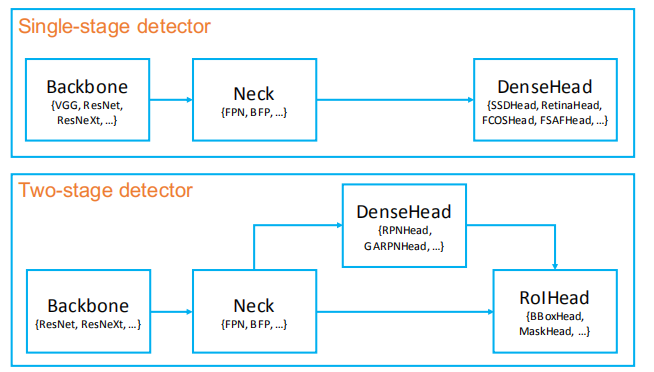
\includegraphics[width=5cm, height=3cm]{./pic/mmdetect.png}
	\caption{ Framework }
	\end{minipage}
	\begin{minipage}[t]{0.48\textwidth}
	\centering
	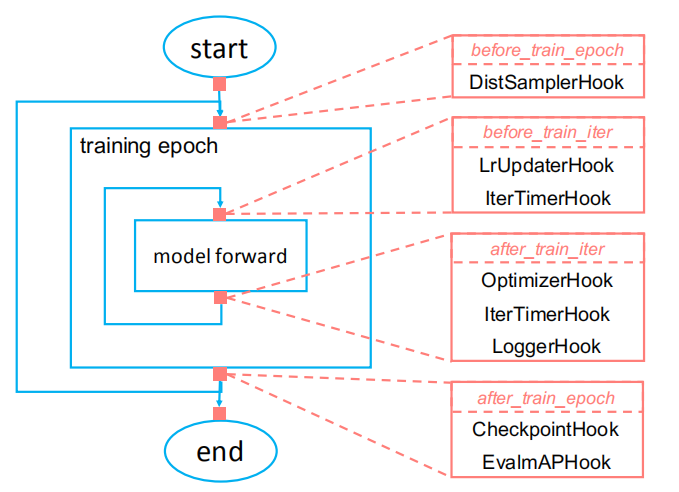
\includegraphics[width=5cm,height=3cm]{./pic/mmdetect_pipe.png}
	\caption{Trainning pipeline}
	\end{minipage}
\end{figure}

% \newpage
\subsection{总体逻辑}
在最外层的train.py中能看到:\\
1. mmcv.Config.fromfile从配置文件解析配置信息,并做适当更新,包括预加载模型文件,分布式相关等\\
2. mmdet.models.builder 中的build\_detector根据配置信息构造模型

\begin{adjustwidth}{0.5cm}{0cm}
2.5 build函数依次遍历配置中的模型信息,调用\_build\_module函数,按type关键字从注册表中获取相应的
模型对象,并根据配置参数实例化对象(配置文件的模型参数只占了各模型构造参数的一小部分,模型结构并非可以随意更改).\\
2.6 registr.py实现了模型的注册装饰器,其主要功能就是将各模型组件类对象保存到registry.module\_dict中,从而可以实现2.5所示功能.\\
2.7 目前包含BACKBONES,NECKS,ROI\_EXTRACTORS,SHARED\_\\
HEADS,HEADS,LOSSES,DETECTORS七个(容器).注册器可按@N
AME.register\_module方式装饰,新增.所有被注册的对象都是一个完整的pytorch构图\
\end{adjustwidth}
3. 最后就是数据迭代器和训练pipeline

\subsection{Configs}
配置方式支持python/json/yaml,从mmcv的Config解析,其功能同maskrcnn-benchmark的yacs类似,将字典的取值方式属性化.

配置文件模型部分包含模型组件及其可改动模型结构的参数,比如backbone的层数,冻结的stage;bbox\_head的in\_channel,类别,损失函数等;训练部分主要包括anchor采样相关系数;测试包括非极大抑制等相关参数;剩下数据,优化器,模型管理,日志等相关信息,一看即明.


\subsection{Backbone}
特征提取,略.
\subsection{Necks}
展开描述:目标尺度和金字塔层级的关系,这些层级对应的尺度与损失函数,样本采样等的关系.
% 要检测到$15\times15$的小目标,有哪些考虑点
\subsection{Heads}
anchor\_heads, bbox\_heads, mask\_heads都将有loss的计算,是核心点,需详细描述.


\subsection{Losses}
选描述
\subsection{Detectors}
重点one\_stage, two\_stage详细阐述

\section{数据处理}
\label{sec:detail}
coco数据等格式,多格式的转换

\section{模型结构}
详细解释一两个模型的细节,比如正负样本采样,损失函数改写,anchor相关尺度变换的细节
\lstset{style=mystyle}
\begin{lstlisting}[language=Python]
import numpy  as np
class Convolution():

	def __init__(self, nc_in, nc_out, kernel_size, stride=2,padding=1):
		self.kernel_size = kernel_size
		self.weights = np.random.randn(nc_in * kernel_size[0] * kernel_size[1] ,nc_out) * np.sqrt(2/nc_in)
		self.biases = np.zeros(nc_out)
		self.stride = stride
		self.padding = padding
	
	def forward(self,x):
		mb, ch, n, p = x.shape
		y = np.matmul(arr2vec(x,self.kernel_size,self.stride,self.padding), self.weights) + self.biases
		y = np.transpose(y,(0,2,1))
		n1 = (n-self.kernel_size[0]+ 2 * self.padding) //self.stride + 1
		p1 = (p-self.kernel_size[1]+2 * self.padding )//self.stride + 1
		return y.reshape(mb,self.biases.shape[0],n1,p1)
	
    def backward(self,grad):
        """
        写点字可以?
        """
		mb, ch_out, n1, p1 = grad.shape
		grad = np.transpose(grad.reshape(mb,ch_out,n1*p1),(0,2,1))
		self.grad_b = grad.sum(axis=1).mean(axis=0)
		self.grad_w = (np.matmul(self.old_x[:,:,:,None],grad[:,:,None,:])).sum(axis=1).mean(axis=0)
		new_grad = np.matmul(grad,self.weights.transpose())
		return vec2arr(new_grad, self.kernel_size, self.old_size, self.stride, self.padding)

\end{lstlisting}
OneStage,TwoStage,其他
\section{训练pipeline}
Hook相关
\section{更改模型}
案例
\section{新增模型}
RetinaFace, BlazeFace, FaceBoxes等

\end{document}